\section{Major Components in our project}

\subsection{Simple Pendulum}
\begin{wrapfigure}{r}{0.4\textwidth}
	\caption{A picture of simple pendulum}
	\begin{center}
	 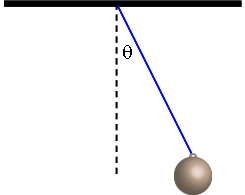
\includegraphics[width=0.2\textwidth]{./doc/pendulum.png}%
	 \end{center}
	
\end{wrapfigure}

\begin{frame}
\centering


\begin{flushleft}

\end{flushleft}
Our project starts with an oscillating simple\\ pendulum giving impulse to a domino placed\\ on one side of it and a ball placed on other side of it.\\ \\ \\ \\ \\
\end{frame}

%%%%%%%%%%%%%%%%%%%%%%%%%%%%%%%%%%%%%%%%%%%%%%%%%%%%%%%%%%%%%%%
\subsection{Conveyor belt}
\begin{wrapfigure}{r}{0.4\textwidth}
	\caption{A picture of conveyor belt}
	\centering
	 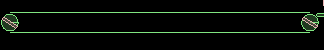
\includegraphics[width=0.2\textwidth]{./doc/conveyor.png}%
\end{wrapfigure}
\begin{frame}
\centering
\\
Conveyor in our project is used to carry\\ a block which triggers a mechanism . \\
Here whenever an object falls on\\ the conveyor belt we used sensors to \\detect the object and give it a force to the \\left or right accordingly.\\We introduced there two rotating motors to\\ give the effect of conveyor belt. 
\end{frame}


%%%%%%%%%%%%%%%%%%%%%%%%%%%%%%%%%%%%%%%%%%%%%%%%%%%%%%%%%%%%%%%
\subsection{Pressure transfering system}
\begin{wrapfigure}{r}{0.4\textwidth}
	\caption{A picture of pressure tranfering system}
	\centering
	 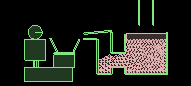
\includegraphics[width=0.2\textwidth]{./doc/pascal.png}%
\end{wrapfigure}
\begin{frame}
\centering
\\
\\
In this system when we give pressure on \\a larger surface on the plunger above popcorn (balls) \\on right using a heavy ball that comes through the channel \\above it. This pressure gets equally\\ distributed and the popcorn (balls)\\ filled inside the box are squeezed. They get pushed and emerge\\ from the left funnel and get delivered into man's bowl to the left \\of the system. This collection of static rectangular objects to the left\\ of this system represents man sitting on chair with a table holding bowl, \\ready to eat things that are delivered from the funnel.
\end{frame}
\\
\\
\\
\\
%%%%%%%%%%%%%%%%%%%%%%%%%%%%%%%%%%%%%%%%%%%%%%%%%%%%%%%%%%%%%%%
\newpage
\subsection{Balloon System}
\begin{wrapfigure}{r}{0.4\textwidth}
	\caption{A picture of balloon system}
	\centering
	 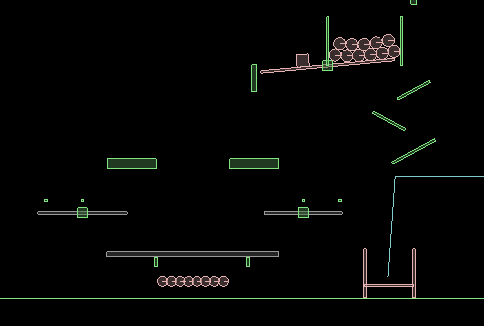
\includegraphics[width=0.2\textwidth]{./doc/balloon.png}%
\end{wrapfigure}
\begin{frame}
\centering
\\
\\
We made this balloon system simulation\\by introducing the negative gravity because of \\which they move upward to trigger \\the few dynamic bodies to get lifted. This will further \\stimulate the balls in upper container to fall \\and stimulate pulley. The upper container containing balls has an \\opening which is blocked by a motor of zero angular velocity and high torque. \\The negative gravity balls slowly accumulate on left pane of the motor and\\ push it so as to unblock the opening and allow the \\balls to fall in pan of pulley.
\end{frame}
\\
\\
%%%%%%%%%%%%%%%%%%%%%%%%%%%%%%%%%%%%%%%%%%%%%%%%%%%%%%%%%%%%%%
\subsection{Rotating Motor}
\begin{wrapfigure}{r}{0.4\textwidth}
	\caption{A picture of rotating motor}
	\centering
	 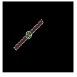
\includegraphics[width=0.2\textwidth]{./doc/motor.jpg}%
\end{wrapfigure}
\begin{frame}
\centering
\\
\\
We have introduced Revolute Joint and enabled \\the motor property.We have given that\\ motor an angular speed and required torque\\ accordingly. Such motors have been used in our project \\to provide required momentum to balls moving along in simulation.
\end{frame}
\\
\\
%%%%%%%%%%%%%%%%%%%%%%%%%%%%%%%%%%%%%%%%%%%%%%%%%%%%%%%%%%
\subsection{Letter S}
\begin{wrapfigure}{r}{0.4\textwidth}
	\caption{A picture of hinge system}
	\centering
	 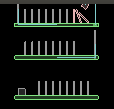
\includegraphics[width=0.2\textwidth]{./doc/S.png}%
\end{wrapfigure}
\begin{frame}
\centering
\\
\\
Basically S letter is made of 3 horizontal planks one below\\ the other, upon which train of dominos is kept.
The topmost \\domino is stimulated by the pendulum described above. \\This leads to a chain reaction making all dominos fall.
We \\implemented Revolute Joint to give the effect of\\ hinge.It takes one anchor and two objects\\ and connects the two objects with the\\ thread through the point.We defined\\ one of the objects as a dynamic rod and other\\ as a small static object with the anchor point\\ on itself which gives the effect\\ of hinge.So, when dominos fall off on the horizontal planks in 'S', the last domino to fall on each plank is hinged in this way to the tip of horizontal plank. So it stays connected to the plank as it dangles down to the area above lower plank. This helps to stimulate dominos on the lower planks successively.
\end{frame}
\\
%%%%%%%%%%%%%%%%%%%%%%%%%%%%%%%%%%%%%%%%%%%%%%%%%%%%%%%%%%%%%
\newpage
\subsection{W letter}
\begin{wrapfigure}{r}{0.4\textwidth}
	\caption{A picture of letter W}
	\centering
	 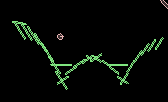
\includegraphics[width=0.2\textwidth]{./doc/W.png}%
\end{wrapfigure}
\begin{frame}
\centering
\\
\\
W letter is basically made of static rectangular blocks \\added according to parabolic trajectory defined by loop variables.\\ This is added
using 4 for-loops and the inclinations, and sizes are \\controlled by the loop variables too. Ultimately 2 horizontal planks\\ are added
at the 2 pointed parts of W letter in the bottom so that \\a ball can bounce over it and move to the next letter.
\end{frame}
\\
\\
\\

\subsection{A Letter}
\begin{wrapfigure}{r}{0.4\textwidth}
	\caption{A picture of letter A}
	\centering
	 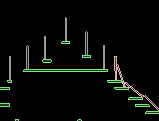
\includegraphics[width=0.2\textwidth]{./doc/A.png}%
\end{wrapfigure}
\begin{frame}
\centering
\\
\\
This is formed using a number of small static horizontal \\planks placed one near the other, and dominos stand over each\\ of these planks.
These dominos are triggered into action due to the\\ block that is delivered by conveyor. They fall one after the other \\revealing an A in the end. The leftmost domino is triggered by block \\delivered by conveyor while the rightmost domino begins to fall by \\itself in the beginning of simulation. This is done by adding small slope \\to the rightmost domino in the constructor function for the \\simulation, so that it is not in balance and falls off making all the \\leftward dominos relative to it fall one after the other.
\end{frame}
\\
\\

%%%%%%%%%%%%%%%%%%%%%%%%%%%%%%%%%%%%%%%%%%%%%%%%%%%%%%%%%%%%%

\subsection{G letter}
\begin{wrapfigure}{r}{0.4\textwidth}
	\caption{A picture of letter G}
	\centering
	 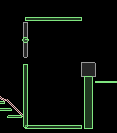
\includegraphics[width=0.2\textwidth]{./doc/G.png}%
\end{wrapfigure}
\begin{frame}
\centering
\\
\\
This letter is formed by a number of static rectangular \\bodies arranged to form this letter. The rightward stem of\\ G holds a dynamic box. There is a motor on left arm of G, which acts \\as a window for the ball which will bounce off from W and enter\\ into the letter G. This is implemented as a revolute joint again. The \\right of G is constructed so as the dynamic box kept on stem of G \\slides off and pushes the heavy ball to its right into action, and the \\heavy ball falls into the tunnel made at the right of G.
\end{frame}
\\
\\
%%%%%%%%%%%%%%%%%%%%%%%%%%%%%%%%%%%%%%%%%%%%%%%%%%%%%%%%%%%%%




\newpage

%%%%%%%%%%%%%%%%%%%%%%%%%%%%%%%%%%%%%%%%%%%%%%%%%%%%%%%%%%%%%
\subsection{Pulley system}
\begin{wrapfigure}{r}{0.4\textwidth}
	\caption{A picture of pulley system}
	\centering
	 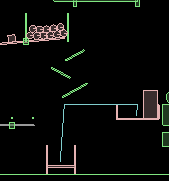
\includegraphics[width=0.2\textwidth]{./doc/pulley.png}%
\end{wrapfigure}
\begin{frame}
\centering
\\
\\
Pulley joints are used to make this system\\which takes two anchors and two objects and \\connects the two objects with the thread\\ through two points giving the effect\\ of a common balance. In our project, the right container is \\successively filled with few balls that are let into it directly. \\This creates downword force, and the pulley joint helps in\\ moving one pan up and the other down.The balls fall \\into left pan of the pulley and \\make the right pan rise up and deliver some more food to the man.
\end{frame}
\\
\\
%%%%%%%%%%%%%%%%%%%%%%%%%%%%%%%%%%%%%%%%%%%%%%%%%%%%%%%%%%%%%


